\chapter{Thuật toán căn bậc hai}

\index{square root algorithm}

Một \key{thuật toán căn bậc hai} là một thuật toán
có căn bậc hai trong độ phức tạp thời gian của nó.
Một căn bậc hai có thể được coi là một "logarit của người nghèo":
độ phức tạp $O(\sqrt n)$ tốt hơn $O(n)$
nhưng tệ hơn $O(\log n)$.
Trong mọi trường hợp, nhiều thuật toán căn bậc hai nhanh và có thể sử dụng được trong thực tế.

Ví dụ, hãy xem xét bài toán
tạo một cấu trúc dữ liệu hỗ trợ
hai thao tác trên một mảng:
sửa đổi một phần tử tại một vị trí cho trước
và tính tổng các phần tử trong một phạm vi cho trước.
Trước đây chúng ta đã giải quyết bài toán này bằng cách sử dụng
cây chỉ số nhị phân và cây phân đoạn,
hỗ trợ cả hai thao tác trong thời gian $O(\log n)$.
Tuy nhiên, bây giờ chúng ta sẽ giải quyết bài toán
theo một cách khác bằng cách sử dụng cấu trúc căn bậc hai
cho phép chúng ta sửa đổi các phần tử trong thời gian $O(1)$
và tính tổng trong thời gian $O(\sqrt n)$.

Ý tưởng là chia mảng thành các \emph{khối}
có kích thước $\sqrt n$ sao cho mỗi khối chứa
tổng các phần tử bên trong khối đó.
Ví dụ, một mảng gồm 16 phần tử sẽ được
chia thành các khối gồm 4 phần tử như sau:

\begin{center}
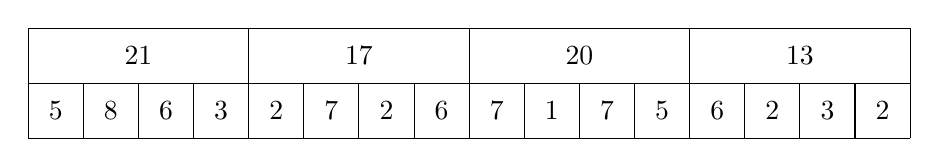
\begin{tikzpicture}[scale=0.7]
\draw (0,0) grid (16,1);

\draw (0,1) rectangle (4,2);
\draw (4,1) rectangle (8,2);
\draw (8,1) rectangle (12,2);
\draw (12,1) rectangle (16,2);

\node at (0.5, 0.5) {5};
\node at (1.5, 0.5) {8};
\node at (2.5, 0.5) {6};
\node at (3.5, 0.5) {3};
\node at (4.5, 0.5) {2};
\node at (5.5, 0.5) {7};
\node at (6.5, 0.5) {2};
\node at (7.5, 0.5) {6};
\node at (8.5, 0.5) {7};
\node at (9.5, 0.5) {1};
\node at (10.5, 0.5) {7};
\node at (11.5, 0.5) {5};
\node at (12.5, 0.5) {6};
\node at (13.5, 0.5) {2};
\node at (14.5, 0.5) {3};
\node at (15.5, 0.5) {2};

\node at (2, 1.5) {21};
\node at (6, 1.5) {17};
\node at (10, 1.5) {20};
\node at (14, 1.5) {13};

\end{tikzpicture}
\end{center}

Trong cấu trúc này,
việc sửa đổi các phần tử mảng rất dễ dàng,
bởi vì chỉ cần cập nhật
tổng của một khối duy nhất
sau mỗi lần sửa đổi,
điều này có thể được thực hiện trong thời gian $O(1)$.
Ví dụ, hình sau cho thấy
cách giá trị của một phần tử và
tổng của khối tương ứng thay đổi:

\begin{center}
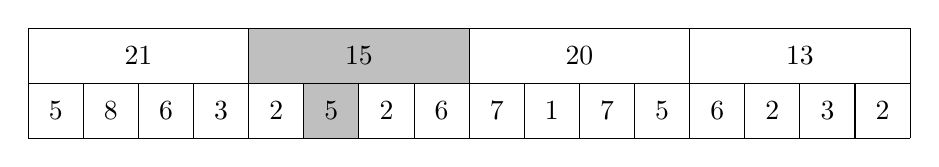
\begin{tikzpicture}[scale=0.7]
\fill[color=lightgray] (5,0) rectangle (6,1);
\draw (0,0) grid (16,1);

\fill[color=lightgray] (4,1) rectangle (8,2);
\draw (0,1) rectangle (4,2);
\draw (4,1) rectangle (8,2);
\draw (8,1) rectangle (12,2);
\draw (12,1) rectangle (16,2);

\node at (0.5, 0.5) {5};
\node at (1.5, 0.5) {8};
\node at (2.5, 0.5) {6};
\node at (3.5, 0.5) {3};
\node at (4.5, 0.5) {2};
\node at (5.5, 0.5) {5};
\node at (6.5, 0.5) {2};
\node at (7.5, 0.5) {6};
\node at (8.5, 0.5) {7};
\node at (9.5, 0.5) {1};
\node at (10.5, 0.5) {7};
\node at (11.5, 0.5) {5};
\node at (12.5, 0.5) {6};
\node at (13.5, 0.5) {2};
\node at (14.5, 0.5) {3};
\node at (15.5, 0.5) {2};

\node at (2, 1.5) {21};
\node at (6, 1.5) {15};
\node at (10, 1.5) {20};
\node at (14, 1.5) {13};

\end{tikzpicture}
\end{center}

Sau đó, để tính tổng các phần tử trong một phạm vi,
chúng ta chia phạm vi thành ba phần sao cho 
tổng bao gồm các giá trị của các phần tử đơn lẻ
và tổng của các khối giữa chúng:

\begin{center}
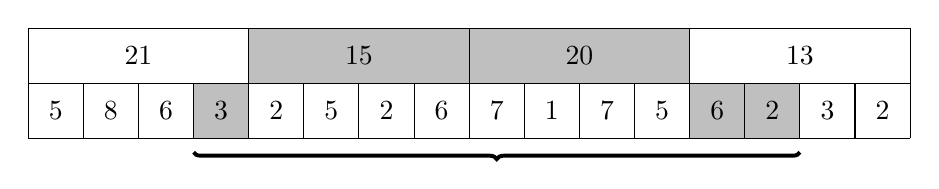
\begin{tikzpicture}[scale=0.7]
\fill[color=lightgray] (3,0) rectangle (4,1);
\fill[color=lightgray] (12,0) rectangle (13,1);
\fill[color=lightgray] (13,0) rectangle (14,1);
\draw (0,0) grid (16,1);

\fill[color=lightgray] (4,1) rectangle (8,2);
\fill[color=lightgray] (8,1) rectangle (12,2);
\draw (0,1) rectangle (4,2);
\draw (4,1) rectangle (8,2);
\draw (8,1) rectangle (12,2);
\draw (12,1) rectangle (16,2);

\node at (0.5, 0.5) {5};
\node at (1.5, 0.5) {8};
\node at (2.5, 0.5) {6};
\node at (3.5, 0.5) {3};
\node at (4.5, 0.5) {2};
\node at (5.5, 0.5) {5};
\node at (6.5, 0.5) {2};
\node at (7.5, 0.5) {6};
\node at (8.5, 0.5) {7};
\node at (9.5, 0.5) {1};
\node at (10.5, 0.5) {7};
\node at (11.5, 0.5) {5};
\node at (12.5, 0.5) {6};
\node at (13.5, 0.5) {2};
\node at (14.5, 0.5) {3};
\node at (15.5, 0.5) {2};

\node at (2, 1.5) {21};
\node at (6, 1.5) {15};
\node at (10, 1.5) {20};
\node at (14, 1.5) {13};

\draw [decoration={brace}, decorate, line width=0.5mm] (14,-0.25) -- (3,-0.25);

\end{tikzpicture}
\end{center}

Vì số lượng phần tử đơn lẻ là $O(\sqrt n)$
và số lượng khối cũng là $O(\sqrt n)$,
truy vấn tổng mất thời gian $O(\sqrt n)$.
Mục đích của kích thước khối $\sqrt n$ là
nó \emph{cân bằng} hai thứ:
mảng được chia thành $\sqrt n$ khối,
mỗi khối chứa $\sqrt n$ phần tử.

Trong thực tế, không cần thiết phải sử dụng
giá trị chính xác của $\sqrt n$ làm tham số,
và thay vào đó chúng ta có thể sử dụng các tham số $k$ và $n/k$ trong đó $k$
khác $\sqrt n$.
Tham số tối ưu phụ thuộc vào bài toán và đầu vào.
Ví dụ, nếu một thuật toán thường xuyên
duyệt qua các khối nhưng hiếm khi kiểm tra
các phần tử đơn lẻ bên trong các khối,
có thể là một ý tưởng tốt để chia mảng thành
$k < \sqrt n$ khối, mỗi khối chứa $n/k > \sqrt n$
phần tử.

\section{Kết hợp các thuật toán}

Trong phần này, chúng ta thảo luận về hai thuật toán căn bậc hai
dựa trên việc kết hợp hai thuật toán thành một thuật toán.
Trong cả hai trường hợp, chúng ta có thể sử dụng một trong hai thuật toán
mà không cần đến thuật toán còn lại
và giải quyết bài toán trong thời gian $O(n^2)$.
Tuy nhiên, bằng cách kết hợp các thuật toán, thời gian
chạy chỉ là $O(n \sqrt n)$.

\subsubsection{Xử lý theo trường hợp}

Giả sử chúng ta được cho một
lưới hai chiều chứa $n$ ô.
Mỗi ô được gán một chữ cái,
và nhiệm vụ của chúng ta là tìm hai ô
có cùng chữ cái mà khoảng cách của chúng là nhỏ nhất,
trong đó khoảng cách giữa các ô
$(x_1,y_1)$ và $(x_2,y_2)$ là $|x_1-x_2|+|y_1-y_2|$.
Ví dụ, hãy xem xét lưới sau:

\begin{center}
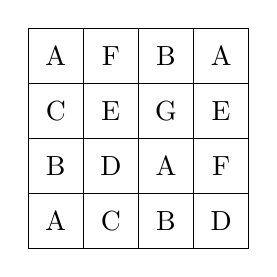
\begin{tikzpicture}[scale=0.7]
\node at (0.5,0.5) {A};
\node at (0.5,1.5) {B};
\node at (0.5,2.5) {C};
\node at (0.5,3.5) {A};
\node at (1.5,0.5) {C};
\node at (1.5,1.5) {D};
\node at (1.5,2.5) {E};
\node at (1.5,3.5) {F};
\node at (2.5,0.5) {B};
\node at (2.5,1.5) {A};
\node at (2.5,2.5) {G};
\node at (2.5,3.5) {B};
\node at (3.5,0.5) {D};
\node at (3.5,1.5) {F};
\node at (3.5,2.5) {E};
\node at (3.5,3.5) {A};
\draw (0,0) grid (4,4);
\end{tikzpicture}
\end{center}
Trong trường hợp này, khoảng cách nhỏ nhất là 2 giữa hai chữ cái 'E'.

Chúng ta có thể giải quyết bài toán bằng cách xem xét từng chữ cái riêng biệt.
Sử dụng cách tiếp cận này, bài toán mới là tính
khoảng cách nhỏ nhất
giữa hai ô có một chữ cái \emph{cố định} $c$.
Chúng ta tập trung vào hai thuật toán cho việc này:

\emph{Thuật toán 1:} Duyệt qua tất cả các cặp ô có chữ cái $c$,
và tính khoảng cách nhỏ nhất giữa các ô đó.
Việc này sẽ mất thời gian $O(k^2)$ trong đó $k$ là số ô có chữ cái $c$.

\emph{Thuật toán 2:} Thực hiện tìm kiếm theo chiều rộng đồng thời
bắt đầu tại mỗi ô có chữ cái $c$. Khoảng cách nhỏ nhất giữa
hai ô có chữ cái $c$ sẽ được tính trong thời gian $O(n)$.

Một cách để giải quyết bài toán là chọn một trong hai
thuật toán và sử dụng nó cho tất cả các chữ cái.
Nếu chúng ta sử dụng Thuật toán 1, thời gian chạy là $O(n^2)$,
bởi vì tất cả các ô có thể chứa cùng một chữ cái,
và trong trường hợp này $k=n$.
Cũng như vậy, nếu chúng ta sử dụng Thuật toán 2, thời gian chạy là $O(n^2)$,
bởi vì tất cả các ô có thể có các chữ cái khác nhau,
và trong trường hợp này cần $n$ lần tìm kiếm.

Tuy nhiên, chúng ta có thể \emph{kết hợp} hai thuật toán và
sử dụng các thuật toán khác nhau cho các chữ cái khác nhau
tùy thuộc vào số lần mỗi chữ cái xuất hiện trong lưới.
Giả sử một chữ cái $c$ xuất hiện $k$ lần.
Nếu $k \le \sqrt n$, chúng ta sử dụng Thuật toán 1, và nếu $k > \sqrt n$,
chúng ta sử dụng Thuật toán 2.
Hóa ra bằng cách làm như vậy, tổng thời gian chạy
của thuật toán chỉ là $O(n \sqrt n)$.

Đầu tiên, giả sử chúng ta sử dụng Thuật toán 1 cho một chữ cái $c$.
Vì $c$ xuất hiện nhiều nhất $\sqrt n$ lần trong lưới,
chúng ta so sánh mỗi ô có chữ cái $c$ $O(\sqrt n)$ lần
với các ô khác.
Do đó, thời gian được sử dụng để xử lý tất cả các ô đó là $O(n \sqrt n)$.
Sau đó, giả sử chúng ta sử dụng Thuật toán 2 cho một chữ cái $c$.
Có nhiều nhất $\sqrt n$ chữ cái như vậy,
vì vậy việc xử lý các chữ cái đó cũng mất thời gian $O(n \sqrt n)$.

\subsubsection{Xử lý theo lô}

Bài toán tiếp theo của chúng ta cũng liên quan đến
một lưới hai chiều chứa $n$ ô.
Ban đầu, mỗi ô ngoại trừ một ô là màu trắng.
Chúng ta thực hiện $n-1$ thao tác, mỗi thao tác trước tiên
tính khoảng cách nhỏ nhất từ một ô trắng cho trước
đến một ô đen, và sau đó tô ô trắng đó thành màu đen.

Ví dụ, hãy xem xét thao tác sau:

\begin{center}
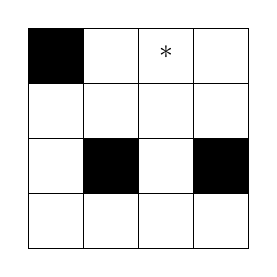
\begin{tikzpicture}[scale=0.7]
\fill[color=black] (1,1) rectangle (2,2);
\fill[color=black] (3,1) rectangle (4,2);
\fill[color=black] (0,3) rectangle (1,4);
\node at (2.5,3.5) {*};
\draw (0,0) grid (4,4);
\end{tikzpicture}
\end{center}

Đầu tiên, chúng ta tính khoảng cách nhỏ nhất
từ ô trắng được đánh dấu * đến một ô đen.
Khoảng cách nhỏ nhất là 2, bởi vì chúng ta có thể di chuyển
hai bước sang trái đến một ô đen.
Sau đó, chúng ta tô ô trắng đó thành màu đen:

\begin{center}
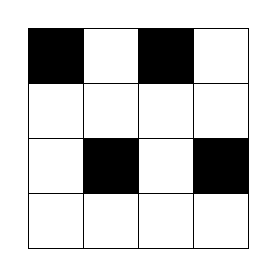
\begin{tikzpicture}[scale=0.7]
\fill[color=black] (1,1) rectangle (2,2);
\fill[color=black] (3,1) rectangle (4,2);
\fill[color=black] (0,3) rectangle (1,4);
\fill[color=black] (2,3) rectangle (3,4);
\draw (0,0) grid (4,4);
\end{tikzpicture}
\end{center}

Hãy xem xét hai thuật toán sau:

\emph{Thuật toán 1:} Sử dụng tìm kiếm theo chiều rộng
để tính
cho mỗi ô trắng khoảng cách đến ô đen gần nhất.
Việc này mất thời gian $O(n)$, và sau khi tìm kiếm,
chúng ta có thể tìm khoảng cách nhỏ nhất từ bất kỳ ô trắng nào
đến một ô đen trong thời gian $O(1)$.

\emph{Thuật toán 2:} Duy trì một danh sách các ô đã được
tô đen, duyệt qua danh sách này ở mỗi thao tác
và sau đó thêm một ô mới vào danh sách.
Một thao tác mất thời gian $O(k)$ trong đó $k$ là độ dài của danh sách.

Chúng ta kết hợp các thuật toán trên bằng cách
chia các thao tác thành
$O(\sqrt n)$ \emph{lô}, mỗi lô bao gồm
$O(\sqrt n)$ thao tác.
Khi bắt đầu mỗi lô,
chúng ta thực hiện Thuật toán 1.
Sau đó, chúng ta sử dụng Thuật toán 2 để xử lý các thao tác
trong lô.
Chúng ta xóa danh sách của Thuật toán 2 giữa
các lô.
Tại mỗi thao tác,
khoảng cách nhỏ nhất đến một ô đen
hoặc là khoảng cách được tính bởi Thuật toán 1
hoặc là khoảng cách được tính bởi Thuật toán 2.

Thuật toán kết quả hoạt động trong
thời gian $O(n \sqrt n)$.
Đầu tiên, Thuật toán 1 được thực hiện $O(\sqrt n)$ lần,
và mỗi lần tìm kiếm hoạt động trong thời gian $O(n)$.
Thứ hai, khi sử dụng Thuật toán 2 trong một lô,
danh sách chứa $O(\sqrt n)$ ô
(bởi vì chúng ta xóa danh sách giữa các lô)
và mỗi thao tác mất thời gian $O(\sqrt n)$.

\section{Phân hoạch số nguyên}

Một số thuật toán căn bậc hai dựa trên
quan sát sau:
nếu một số nguyên dương $n$ được biểu diễn dưới dạng
tổng của các số nguyên dương,
thì một tổng như vậy luôn chứa nhiều nhất
$O(\sqrt n)$ số \emph{phân biệt}.
Lý do cho điều này là để xây dựng
một tổng chứa số lượng tối đa các số phân biệt,
chúng ta nên chọn các số \emph{nhỏ}.
Nếu chúng ta chọn các số $1,2,\ldots,k$,
tổng kết quả là
\[\frac{k(k+1)}{2}.\]
Do đó, số lượng tối đa các số phân biệt là $k = O(\sqrt n)$.
Tiếp theo chúng ta sẽ thảo luận về hai bài toán có thể được giải quyết
một cách hiệu quả bằng cách sử dụng quan sát này.

\subsubsection{Cái túi (Knapsack)}

Giả sử chúng ta được cho một danh sách các trọng lượng số nguyên
có tổng là $n$.
Nhiệm vụ của chúng ta là tìm ra tất cả các tổng có thể được tạo thành bằng cách sử dụng
một tập hợp con các trọng lượng. Ví dụ, nếu các trọng lượng là
$\{1,3,3\}$, các tổng có thể là:

\begin{itemize}[noitemsep]
\item $0$ (tập rỗng)
\item $1$
\item $3$
\item $1+3=4$
\item $3+3=6$
\item $1+3+3=7$
\end{itemize}

Sử dụng cách tiếp cận cái túi tiêu chuẩn (xem Chương 7.4),
bài toán có thể được giải quyết như sau:
chúng ta định nghĩa một hàm $\texttt{possible}(x,k)$ có giá trị là 1
nếu tổng $x$ có thể được tạo thành bằng cách sử dụng $k$ trọng lượng đầu tiên,
và 0 nếu không.
Vì tổng các trọng lượng là $n$,
có nhiều nhất $n$ trọng lượng và
tất cả các giá trị của hàm có thể được tính
trong thời gian $O(n^2)$ bằng cách sử dụng quy hoạch động.

Tuy nhiên, chúng ta có thể làm cho thuật toán hiệu quả hơn
bằng cách sử dụng thực tế là có nhiều nhất $O(\sqrt n)$
trọng lượng \emph{phân biệt}.
Do đó, chúng ta có thể xử lý các trọng lượng theo nhóm
bao gồm các trọng lượng tương tự.
Chúng ta có thể xử lý mỗi nhóm
trong thời gian $O(n)$, mang lại một thuật toán thời gian $O(n \sqrt n)$.

Ý tưởng là sử dụng một mảng ghi lại các tổng trọng lượng
có thể được tạo thành bằng cách sử dụng các nhóm đã được xử lý cho đến nay.
Mảng chứa $n$ phần tử: phần tử $k$ là 1 nếu tổng
$k$ có thể được tạo thành và 0 nếu không.
Để xử lý một nhóm trọng lượng, chúng ta quét mảng
từ trái sang phải và ghi lại các tổng trọng lượng mới
có thể được tạo thành bằng cách sử dụng nhóm này và các nhóm trước đó.

\subsubsection{Xây dựng chuỗi}

Cho một chuỗi \texttt{s} có độ dài $n$
và một tập hợp các chuỗi $D$ có tổng độ dài là $m$,
hãy xem xét bài toán đếm số cách
\texttt{s} có thể được tạo thành dưới dạng một chuỗi ghép
của các chuỗi trong $D$.
Ví dụ,
nếu $\texttt{s}=\texttt{ABAB}$ và
$D=\{\texttt{A},\texttt{B},\texttt{AB}\}$,
có 4 cách:

\begin{itemize}[noitemsep]
\item $\texttt{A}+\texttt{B}+\texttt{A}+\texttt{B}$
\item $\texttt{AB}+\texttt{A}+\texttt{B}$
\item $\texttt{A}+\texttt{B}+\texttt{AB}$
\item $\texttt{AB}+\texttt{AB}$
\end{itemize}

Chúng ta có thể giải quyết bài toán bằng quy hoạch động:
Gọi $\texttt{count}(k)$ là số cách để xây dựng tiền tố
$\texttt{s}[0 \ldots k]$ bằng cách sử dụng các chuỗi trong $D$.
Bây giờ $\texttt{count}(n-1)$ cho ra câu trả lời cho bài toán,
và chúng ta có thể giải quyết bài toán trong thời gian $O(n^2)$
sử dụng cấu trúc trie.

Tuy nhiên, chúng ta có thể giải quyết bài toán hiệu quả hơn
bằng cách sử dụng băm chuỗi và thực tế là có
nhiều nhất $O(\sqrt m)$ độ dài chuỗi phân biệt trong $D$.
Đầu tiên, chúng ta xây dựng một tập hợp $H$ chứa tất cả
các giá trị băm của các chuỗi trong $D$.
Sau đó, khi tính một giá trị của $\texttt{count}(k)$,
chúng ta duyệt qua tất cả các giá trị của $p$
sao cho có một chuỗi có độ dài $p$ trong $D$,
tính giá trị băm của $\texttt{s}[k-p+1 \ldots k]$
và kiểm tra xem nó có thuộc $H$ hay không.
Vì có nhiều nhất $O(\sqrt m)$ độ dài chuỗi phân biệt,
điều này dẫn đến một thuật toán có thời gian chạy là $O(n \sqrt m)$.

\section{Thuật toán của Mo (Mo's algorithm)}

\index{Mo's algorithm}

\key{Thuật toán của Mo (Mo's algorithm)}\footnote{Theo \cite{cod15}, thuật toán này
được đặt theo tên của Mo Tao, một lập trình viên thi đấu người Trung Quốc, nhưng
kỹ thuật này đã xuất hiện trước đó trong tài liệu \cite{ken06}.}
có thể được sử dụng trong nhiều bài toán
yêu cầu xử lý các truy vấn phạm vi trong 
một mảng \emph{tĩnh}, tức là các giá trị mảng
không thay đổi giữa các truy vấn.
Trong mỗi truy vấn, chúng ta được cho một phạm vi $[a,b]$,
và chúng ta nên tính một giá trị dựa trên
các phần tử mảng giữa các vị trí $a$ và $b$.
Vì mảng là tĩnh,
các truy vấn có thể được xử lý theo bất kỳ thứ tự nào,
và thuật toán của Mo
xử lý các truy vấn theo một thứ tự đặc biệt đảm bảo
thuật toán hoạt động hiệu quả.

Thuật toán của Mo duy trì một \emph{phạm vi hoạt động}
của mảng, và câu trả lời cho một truy vấn
liên quan đến phạm vi hoạt động được biết tại mọi thời điểm.
Thuật toán xử lý các truy vấn từng cái một,
và luôn di chuyển các điểm cuối của
phạm vi hoạt động bằng cách chèn và xóa các phần tử.
Độ phức tạp thời gian của thuật toán là
$O(n \sqrt n f(n))$ trong đó mảng chứa
$n$ phần tử, có $n$ truy vấn
và mỗi lần chèn và xóa một phần tử
mất thời gian $O(f(n))$.

Bí quyết trong thuật toán của Mo là thứ tự
mà các truy vấn được xử lý:
Mảng được chia thành các khối gồm $k=O(\sqrt n)$
phần tử, và một truy vấn $[a_1,b_1]$
được xử lý trước một truy vấn $[a_2,b_2]$
nếu
\begin{itemize}
\item $\lfloor a_1/k \rfloor < \lfloor a_2/k \rfloor$ hoặc
\item $\lfloor a_1/k \rfloor = \lfloor a_2/k \rfloor$ và $b_1 < b_2$.
\end{itemize}

Do đó, tất cả các truy vấn có điểm cuối bên trái
trong một khối nhất định được xử lý lần lượt
được sắp xếp theo điểm cuối bên phải của chúng.
Sử dụng thứ tự này, thuật toán
chỉ thực hiện $O(n \sqrt n)$ thao tác,
bởi vì điểm cuối bên trái di chuyển
$O(n)$ lần $O(\sqrt n)$ bước,
và điểm cuối bên phải di chuyển
$O(\sqrt n)$ lần $O(n)$ bước. Do đó, cả hai
điểm cuối di chuyển tổng cộng $O(n \sqrt n)$ bước trong suốt thuật toán.

\subsubsection*{Ví dụ}

Ví dụ, hãy xem xét một bài toán
trong đó chúng ta được cho một tập hợp các truy vấn,
mỗi truy vấn tương ứng với một phạm vi trong một mảng,
và nhiệm vụ của chúng ta là tính cho mỗi truy vấn
số lượng các phần tử \emph{phân biệt} trong phạm vi đó.

Trong thuật toán của Mo, các truy vấn luôn được sắp xếp
theo cùng một cách, nhưng việc
duy trì câu trả lời cho truy vấn phụ thuộc vào bài toán.
Trong bài toán này, chúng ta có thể duy trì một mảng 
\texttt{count} trong đó $\texttt{count}[x]$
chỉ ra số lần một phần tử $x$
xuất hiện trong phạm vi hoạt động.

Khi chúng ta di chuyển từ một truy vấn này sang một truy vấn khác,
phạm vi hoạt động thay đổi.
Ví dụ, nếu phạm vi hiện tại là
\begin{center}
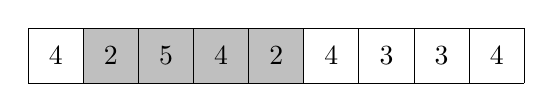
\begin{tikzpicture}[scale=0.7]
\fill[color=lightgray] (1,0) rectangle (5,1);
\draw (0,0) grid (9,1);
\node at (0.5, 0.5) {4};
\node at (1.5, 0.5) {2};
\node at (2.5, 0.5) {5};
\node at (3.5, 0.5) {4};
\node at (4.5, 0.5) {2};
\node at (5.5, 0.5) {4};
\node at (6.5, 0.5) {3};
\node at (7.5, 0.5) {3};
\node at (8.5, 0.5) {4};
\end{tikzpicture}
\end{center}
và phạm vi tiếp theo là
\begin{center}
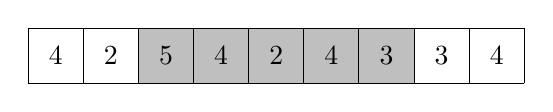
\begin{tikzpicture}[scale=0.7]
\fill[color=lightgray] (2,0) rectangle (7,1);
\draw (0,0) grid (9,1);
\node at (0.5, 0.5) {4};
\node at (1.5, 0.5) {2};
\node at (2.5, 0.5) {5};
\node at (3.5, 0.5) {4};
\node at (4.5, 0.5) {2};
\node at (5.5, 0.5) {4};
\node at (6.5, 0.5) {3};
\node at (7.5, 0.5) {3};
\node at (8.5, 0.5) {4};
\end{tikzpicture}
\end{center}
sẽ có ba bước:
điểm cuối bên trái di chuyển một bước sang phải,
và điểm cuối bên phải di chuyển hai bước sang phải.

Sau mỗi bước, mảng \texttt{count}
cần được cập nhật.
Sau khi th

êm một phần tử $x$,
chúng ta tăng giá trị của 
$\texttt{count}[x]$ lên 1,
và nếu $\texttt{count}[x]=1$ sau đó,
chúng ta cũng tăng câu trả lời cho truy vấn lên 1.
Tương tự, sau khi xóa một phần tử $x$,
chúng ta giảm giá trị của 
$\texttt{count}[x]$ đi 1,
và nếu $\texttt{count}[x]=0$ sau đó,
chúng ta cũng giảm câu trả lời cho truy vấn đi 1.

Trong bài toán này, thời gian cần thiết để thực hiện
mỗi bước là $O(1)$, vì vậy tổng độ phức tạp thời gian
của thuật toán là $O(n \sqrt n)$.